\let\lesson\undefined
\newcommand{\lesson}{\phantomlesson{Bài 1 + 2: Khái quát về môn Vật lí - Vấn đề an toàn trong Vật lí}}
\chapter[Khái quát về môn Vật lí - Vấn đề an toàn trong Vật lí]{Khái quát về môn Vật lí - Vấn đề an toàn trong Vật lí}
\section{Lý thuyết}
%\subsection{Các đơn vị thường dùng trong vật lí học}
%\subsubsection{Đơn vị cơ bản}
%\begin{longtable}{|c|m{11em}|m{13em}|m{8em}|}
%	\hline
%	\thead{TT} & \thead{Đại lượng} & \thead{Tên đơn vị} & \thead{Kí hiệu đơn vị}
%	\\
%	\hline	
%	1 & Độ dài & mét & m 
%	\\
%	\hline	
%	2 & Khối lượng & kilôgam & kg
%	\\
%	\hline	
%	3 & Thời gian & giây & s
%	\\
%	\hline	
%	4 & Cường độ dòng điện & ampe & A 
%	\\
%	\hline	
%	5 & Nhiệt độ & kenvin & K
%	\\
%	\hline	
%	6 & Lượng chất & mol & mol
%	\\
%	\hline	
%	7 & Cường độ sáng & candela & cd
%	\\
%	\hline	

%\end{longtable}
%\subsubsection{Đơn vị dẫn xuất}
%\begin{longtable}{|c|m{11em}|m{13em}|m{8em}|}
%	\hline
%	\thead{TT} & \thead{Đại lượng} & \thead{Tên đơn vị} & \thead{Kí hiệu đơn vị}
%	\\
%	\hline	
%	\multicolumn{4}{|c|}{\textbf{Đơn vị không gian, thời gian và hiện tượng tuần hoàn}}
%	\\
%	\hline	
%	1 & Góc phẳng & rađian & rad 
%	\\
%	\hline	
%	2 & Diện tích & mét vuông & m$^2$
%	\\
%	\hline	
%	3 & Thể tích & mét khối & m$^3$
%	\\
%	\hline	
%	4 & Tần số & héc & Hz 
%	\\
%	\hline	
%	5 & Vận tốc góc & rađian trên giây & rad/s
%	\\
%	\hline	
%	6 & Gia tốc góc & rađian trên giây bình phương & rad/s$^2$
%	\\
%	\hline	
%	7 & Vận tốc & mét trên giây & m/s
%	\\
%	\hline	
%	8 & Gia tốc & mét trên giây bình phương & m/s$^2$
%	\\
%	\hline	
%		\multicolumn{4}{|c|}{\textbf{Đơn vị cơ}}
%	\\
%	\hline	
%	9 & Khối lượng riêng & kilôgam trên mét khối & kg/m$^3$ 
%	\\
%	\hline	
%	10 & Lực & niutơn & N
%	\\
%	\hline	
%	11 & Moment lực & niutơn mét & \SI{}{\newton.\meter}
%	\\
%	\hline	
%	12 & Áp suất & pascan & Pa 
%	\\
%	\hline	

%\end{longtable}

\subsection{Đối tượng - Mục tiêu - Phương pháp nghiên cứu Vật lý}
\subsubsection{Đối tượng nghiên cứu của vật lí}
Vật lí là môn ``khoa học tự nhiên'' có đối tượng nghiên cứu tập trung vào các dạng vận động của vật chất (chất, trường), năng lượng.
\subsubsection{Mục tiêu học tập môn vật lí}
Mục tiêu của vật lí là khám phá ra quy luật tổng quát nhất chi phối sự vận động của vật chất và năng lượng cũng như tương tác giữa chúng ở mọi cấp độ: vi mô, vĩ mô và siêu vĩ mô.
\subsection{Quá trình phát triển của vật lí}
\begin{center}
	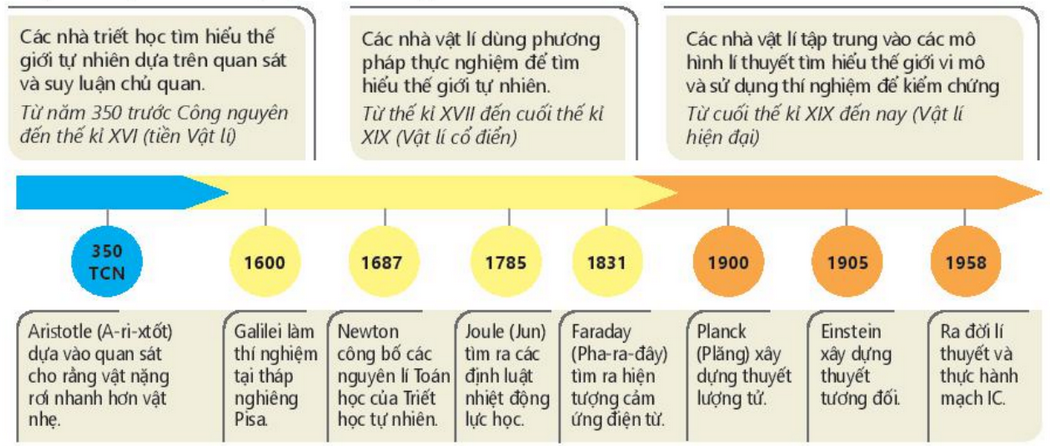
\includegraphics[width=0.95\textwidth]{../figs/G10-1-1}
\end{center}
\subsection{Phương pháp nghiên cứu của Vật lí}
Phương pháp nghiên cứu của Khoa học nói chung và Vật lí nói riêng được hình thành qua các thời kì phát triển của nền văn minh nhân loại, bao gồm hai phương pháp chính:
\begin{itemize}
	\item \textbf{\textit{Phương pháp thực nghiệm:}} dùng thí nghiệm để phát hiện kết quả mới giúp kiểm chứng, hoàn thiện, bổ sung hay bác bỏ giả thuyết nào đó. Kết quả mới này cần được giải thích bằng lí thuyết đã biết hoặc lí thuyết mới.
	\item \textbf{\textit{Phương pháp lí thuyết:}} sử dụng ngôn ngữ toán học và suy luận lí thuyết để phát hiện một kết quả mới. Kết quả mới này cần được kiểm chứng bằng thực nghiệm.
\end{itemize}
Hai phương pháp hỗ trợ cho nhau, trong đó phương pháp thực nghiệm có tính quyết định.\\
\textbf{Quy trình tìm hiểu thế giới tự nhiên dưới góc độ Vật lí}
\begin{center}
	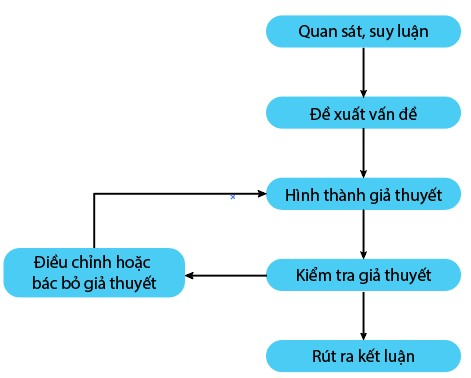
\includegraphics[width=0.6\linewidth]{../figs/VN10-2023-PH-TP002-1}
\end{center}
\subsection{Vai trò của vật lí đối với khoa học, kĩ thuật và công nghệ}
Vật Lý có quan hệ với mọi ngành khoa học và thường được coi là cơ sở của khoa học tự nhiên.

Ảnh hưởng của Vật Lý đến đời sống và kỹ thuật là vô cùng to lớn.
\subsubsection{Thông tin liên lạc}
Ngày nay, khoảng cách địa lí không còn là vấn đề quá lớn của con người trong thông tin liên lạc, sự bùng nổ của mạng lưới internet kết hợp sự phát triển vượt bậc của điện thoại thông minh (smartphone) giúp con người có thể chia sẻ thông tin liên lạc (hình ảnh, giọng nói, tin tức...) một cách dễ dàng. Thế giới ngày này là một thế giới “phẳng”.
\subsubsection{Y tế}
Hầu hết các phương pháp chuẩn đoán và chữa bệnh trong y học đều có cơ sở từ những kiến thức Vật Lý như: chụp X – quang, chụp cộng hưởng từ (MRI), siêu âm, nội soi, xạ trị, \dots
\subsubsection{Công nghiệp}
Cuộc cách mạng công nghiệp lần thứ tư được coi là bắt đầu thế kỉ XXI. Các nền sản xuất thủ công nhỏ lẻ được thay thế bởi những dây chuyền sản xuất tự động hóa, sử dụng trí tuệ nhân tạo, công nghệ vật liệu (nano), điện toán đám mây.
\subsubsection{Nông nghiệp}
Việc ứng dụng những thành tựu của Vật Lý vào nông nghiệp đã giúp cho người nông dân tiếp cận với nhiều phương pháp mới, ít tốn lao động, cho năng suất cao. 
\subsubsection{Nghiên cứu khoa học}
Vật lý góp phần to lớn trong việc cải tiến các thiết bị nghiên cứu khoa học ở nhiều ngành khác nhau như: kính hiển vi điện tử, nhiễu xạ tia X, máy quang phổ, \dots

\subsection{Một số quy định về an toàn trong phòng thực hành vật lí}
\subsubsection{Quy tắc an toàn trong sử dụng các thiết bị điện}
Cần quan sát kĩ các kí hiệu và nhãn thông số trên thiết bị để sử dụng đúng chức năng, đúng yêu cầu kĩ thuật.

Một số kí hiệu trên các thiết bị thí nghiệm:
\begin{center}
	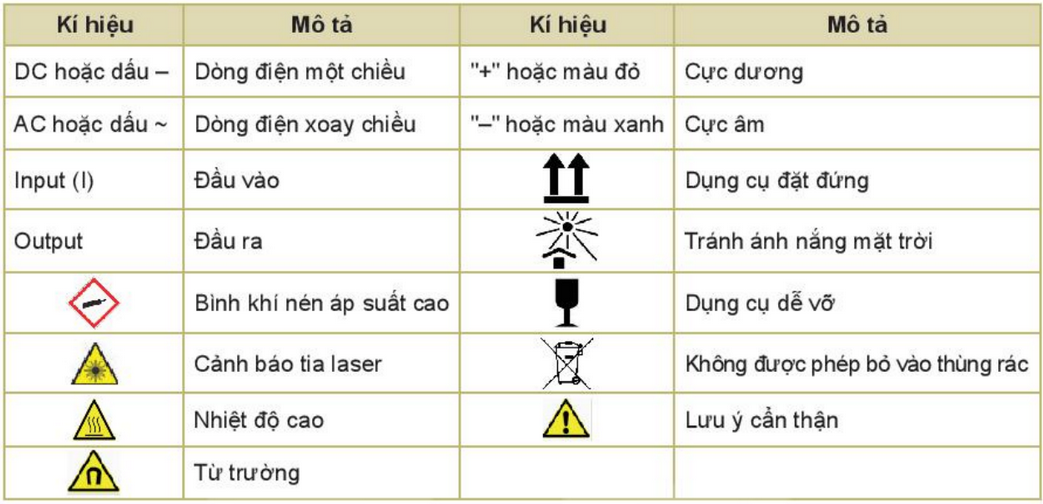
\includegraphics[scale=0.7]{../figs/G10-2-1}
\end{center}
\subsubsection{Quy tắc an toàn sử dụng các thiết bị nhiệt và thủy tinh}
Các thiết bị đun nóng có thể gây cháy hoặc nứt, vỡ các dụng cụ bằng thuỷ tinh.
\subsubsection{Quy tắc an toàn sử dụng các thiết bị quang học}
Các thiết bị quang học rất dễ bị mốc, xước, nứt, vỡ và dính bụi bẩn, làm ảnh hưởng đến đường truyền tia sáng và sai lệch kết quả thí nghiệm.
\section{Mục tiêu bài học - Ví dụ minh họa}
\begin{dang}{Nêu được đối tượng nghiên cứu của\\ vật lí học và mục tiêu của môn Vật lí}
	\viduii{1}{Hãy kể tên các lĩnh vực vật lí mà em đã được học ở cấp Trung học cơ sở.
	}
	{	\begin{center}
			\textbf{Hướng dẫn giải}
		\end{center}
		
		Ở cấp Trung học cơ sở, vật lí nghiên cứu các vấn đề cơ bản nhất của vật lí học, có thể kể đến như:
		\begin{itemize}
			%		\item Đo lường và các dụng cụ đo lường;
			\item Cơ học: Các chuyển động cơ học đơn giản, chuyển động dưới tác dụng của lực, năng lượng cơ học (cơ năng);
			\item Nhiệt học: Các đại lượng đặc trưng trong nhiệt học;
			\item Âm học: Các hiện tượng liên quan đến âm thanh;
			\item Điện học: Các mạch điện chứa điện trở, định luật cơ bản trong điện học;
			\item Quang học: Các dụng cụ quang học thường gặp, các định luật quang hình học.
		\end{itemize}
	}
	\viduii{1}{Học tốt môn vật lí sẽ giúp ích gì cho em?
	}
	{	\begin{center}
			\textbf{Hướng dẫn giải}
		\end{center}
		
		Em hãy trao đổi với giáo viên và bày tỏ suy nghĩ của mình.
	}
\end{dang}

\begin{dang}{Phân tích được một số ảnh hưởng của vật lí đối với cuộc sống, đối với sự phát triển của khoa học, công nghệ và kĩ thuật}
	\viduii{1}{Lấy ví dụ chứng tỏ tri thức vật lí giúp tránh được nguy cơ tổn hại về sức khỏe.
	}
	{	\begin{center}
			\textbf{Hướng dẫn giải}
		\end{center}
		
		Các em có thể lấy ví dụ vào các lĩnh vực nằm trong hiểu biết của mình:
		\begin{itemize}
			\item Kỹ thuật: chế tạo các công cụ, máy móc giúp tiết kiệm sức lao động;
			\item Công nghệ: chế tạo robot để thực hiện những công việc nguy hiểm;
			\item Y sinh: phẫu thuật Laser, nội soi, làm đẹp và thẫm mỹ, $\ldots$; 
			\item Y học dự phòng: thói quen sinh hoạt, làm việc khoa học dựa trên hoạt động của cơ, xương khớp;
			\item Vật lí trị liệu: kích hoạt huyệt đạo trên cơ thể bằng dòng điện, châm cứu, hồng ngoại, tử ngoại, $\ldots$.
		\end{itemize}
	}
	\viduii{1}{Lấy ví dụ và phân tích ảnh hưởng của vật lí đối với sự phát triển của khoa học kĩ thuật và công nghệ
	}
	{\begin{center}
			\textbf{Hướng dẫn giải}
		\end{center}
		
		Các em có thể lấy ví dụ vào các lĩnh vực nằm trong hiểu biết của mình:
		\begin{itemize}
			\item Công nghiệp: máy móc công nghiệp hoạt động dựa trên các nguyên lí về dòng điện và từ trường;
			\item Nông nghiệp: hệ thống chăm sóc nông nghiệp tự động hóa dựa trên các nghiên cứu lượng tử.
			\item Dịch vụ: y tế, đời sống xã hội, giao thông, $\ldots$.
		\end{itemize}
	}
\end{dang}

\begin{dang}{Nêu được ví dụ về các phương pháp nghiên cứu vật lí}
	\viduii{2}
	{Vào đầu thế kỉ XX, J.J.Thomson đã đề xuất mô hình cấu tạo nguyên tử gồm các electron phân bố đều trong một khối điện dương kết cấu tựa như khối mây. Để kiểm chứng giả thuyết này, E. Rutherford đã sử dụng tia alpha gồm các hạt mang điện dương bắn vào các nguyên tử kim loại vàng Hình \ref{fig:2.2}. Kết quả của thí nghiệm đã bác bỏ giả thuyết của J. J. Thomson, đồng thời đã giúp khám phá ra hạt nhân nguyên tử. E. Rutherford đã vận dụng phương pháp nghiên cứu nào để nghiên cứu vấn đề này? Giải thích.
	\begin{center}
		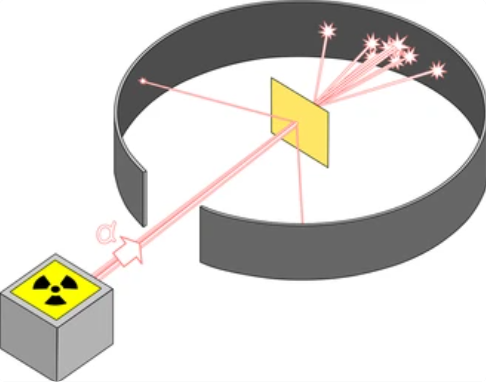
\includegraphics[width=0.3\linewidth]{../figs/VN10-2023-PH-TP002-2}
		\captionof{figure}{Thí nghiệm Rutherford.}
		\label{fig:2.2}
\end{center}  }
	{\begin{center}
			\textbf{Hướng dẫn giải}
		\end{center}
		Rutherford đã sử dụng phương pháp thực nghiệm trong nghiên cứu vật lí vì ông đã thực hiện thí nghiệm dùng tia alpha gồm các hạt mang điện dương bắn vào các nguyên tử vàng để phát hiện ra kết quả mới chính là hạt nhân nguyên tử.
	}
\end{dang}
\begin{dang}{Mô tả được các bước \\trong tiến trình tìm hiểu thế giới tự nhiên}
	\viduii{1}
	{Sắp xếp các bước tiến hành quá trình tìm hiểu thế giới tự nhiên dưới góc độ vật lí:\\
	\begin{enumerate}[label= (\arabic*)]
		\item Phân tích số liệu.
		\item Quan sát, xác định đối tượng cần nghiên cứu.
		\item Thiết kế, xây dựng mô hình kiểm chứng giả thuyết.
		\item Đề xuất giả thuyết nghiên cứu.
		\item Rút ra kết luận.
\end{enumerate} }
	{\begin{center}
			\textbf{Hướng dẫn giải}
		\end{center}
	Tiến trình tìm hiểu thế giới tự nhiên dưới góc độ Vật lí là (2) - (4) - (3) - (1) - (5).
	}
\end{dang}


\begin{dang}{Vận dụng được các quy tắc an toàn \\trong phòng thực hành vật lí}
	\viduii{2}{Hãy nêu quy tắc an toàn trong việc sử dụng các thiết bị sau:
		\begin{enumerate}
			\item Phích cắm điện;
			\item Dây điện;
			\item Nguồn tia LASER;
			\item Đèn cồn.
		\end{enumerate}
	}
	{	\begin{center}
			\textbf{Hướng dẫn giải}
		\end{center}
		
		\begin{enumerate}
			\item Phích cắm điện: Không chạm tay vào vị trí tiếp xúc giữa phích cắm và ổ điện, không cắm điện khi tay ướt.
			\item Dây điện: Không sử dụng dây điện cũ, không đấu nối dây điện thiếu an toàn.
			\item Nguồn tia LASER: Không đặt mắt trực tiếp trên đường truyền của tia LASER, không chiếu tia LASER vào người khác;
			\item Đèn cồn: Không bỏ đi nơi khác khi đang đun bằng đèn cồn, hơ lửa đều để ống nghiệm giãn nở đều.
		\end{enumerate}
	}
	\viduii{2}{Hãy cho biết các dụng cụ đo sau có chức năng gì và cách nối chúng vào mạch điện:
		\begin{enumerate}
			\item Ampe kế;
			\item Vôn kế;
			\item Đồng hồ đo điện đa năng.
		\end{enumerate}
	}
	{\begin{center}
			\textbf{Hướng dẫn giải}
		\end{center}
		
		\begin{enumerate}
			\item Ampe kế: Dùng để đo cường độ dòng điện, nối tiếp với đoạn mạch cần đo;
			\item Vôn kế: Dùng để đo hiệu điện thế, mắc song song với đoạn mạch cần đo;
			\item Đồng hồ đo điện đa năng: Dùng để đo hiệu điện thế, cường độ dòng điện và điện trở, cần vặn núm xoay vào thang đo phù hợp trước khi tiến hành đo.
		\end{enumerate}
	}
\end{dang}
